\section{\texorpdfstring{Ellipsometric angles $\psi$ and $\Delta$}{Ellipsometric angles psi and Delta}}

Ellipsometry measures not reflectances but the complex ratio of the
$p$- and $s$-reflection amplitudes, which carries both amplitude and phase
information. This example evaluates that ratio on two stacks at a fixed
wavelength $\lambda = \SI{633}{\nano\metre}$ (He--Ne): a bare silicon
half-space and a \SI{25}{\nano\metre} oxide film on silicon. The
refractive indices are
$n_{\rm air} = 1.00$,
$n_{\rm SiO_2} = 1.457$ and
$n_{\rm Si} = 3.882 + 0.019\,\ii$. For the bare case the stack is
reduced to the two half-spaces air\,/\,Si; for the covered case it is the
three-layer air\,/\,SiO$_2$\,/\,Si with
$d_{\rm SiO_2} = \SI{25}{\nano\metre}$. The angle of incidence $\theta_0$
is scanned from \SI{0.1}{\degree} to \SI{89}{\degree} on 451 points.

The TMM returns the complex amplitudes $r_s$ and $r_p$ directly, and the
ellipsometric ratio is defined in the standard way,
\begin{equation}
  \rho = \frac{r_p}{r_s} = \tan\psi\,e^{\ii\Delta}, \label{eq:elli-rho}
\end{equation}
so that the two real ellipsometric angles are
\begin{equation}
  \tan\psi = |\rho|,\qquad \Delta = \arg\rho\,\bmod\,2\pi. \label{eq:elli-psi-delta}
\end{equation}
The code uses the sign convention $r_s(0) = r_p(0)$, so $\rho$ computed
directly from the TMM differs from the textbook definition (in which
$\rho = -r_p^{\rm Wiki}/r_s$) by an overall sign; for the bare Si overlay,
the Wikipedia-form analytic $r_p$ is negated once before being fed into
equations~\eqref{eq:elli-rho}--\eqref{eq:elli-psi-delta} so that all
curves are plotted in the same $(\psi, \Delta)$ coordinate system.

Panels (a) and (b) plot $\psi(\theta_0)$ and $\Delta(\theta_0)$ for the
two stacks, with the closed-form Fresnel curves for bare Si overlaid as a
dashed reference. Panel (c) demonstrates the classical inverse problem of
ellipsometry: assuming $n_{\rm SiO_2}$ and $n_{\rm Si}$ are known, the
oxide thickness is reconstructed from the same TMM $(\psi, \Delta)$ data
by minimising the fit residual
\begin{equation}
  \chi^{2}(d) = \sum_{k}\left[\psi_{\rm TMM}(\theta_k) - \psi_d(\theta_k)\right]^{2} + \left[\Delta_{\rm TMM}(\theta_k) - \Delta_d(\theta_k)\right]^{2}, \label{eq:elli-chi2}
\end{equation}
where $(\psi_d, \Delta_d)$ are the TMM predictions for a trial thickness
$d$. The minimisation uses a bounded one-dimensional search on
$d \in [\SI{0}, \SI{100}{\nano\metre}]$ with the measurement grid
$\theta_k \in [\SI{50}, \SI{85}{\degree}]$ (71 points), chosen to cover the
angular range where $\Delta$ is most sensitive to the oxide thickness.

\begin{center}
\begin{tikzpicture}
  \fill[black!4] (0, 0) rectangle (5, 1.4);
  \fill[green!10] (0,-0.5) rectangle (5, 0);
  \fill[blue!6]  (0,-1.7) rectangle (5,-0.5);
  \draw[thick] (0,0) -- (5,0);
  \draw[thick] (0,-0.5) -- (5,-0.5);
  \node[lbl, anchor=east] at (4.9, 1.0) {air};
  \node[lbl, anchor=east] at (4.9,-0.25) {SiO$_2$, $d$};
  \node[lbl, anchor=east] at (4.9,-1.1) {Si};
  \raysketch{1.6}{55}{f}
\end{tikzpicture}
\end{center}

\begin{figure}[!htbp]
  \centering
  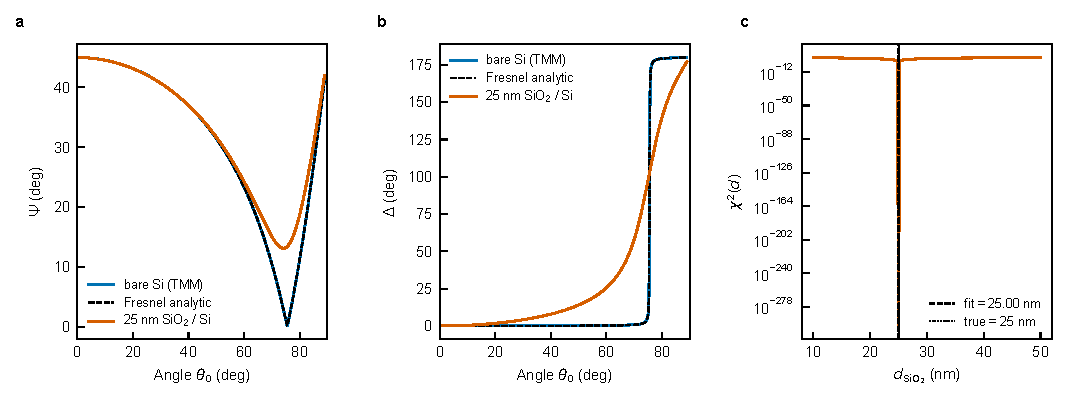
\includegraphics[width=\textwidth]{14_ellipsometry_psi_delta.pdf}
  \caption{Ellipsometric angles at \SI{633}{\nano\metre} for bare Si and for \SI{25}{\nano\metre} SiO$_2$/Si. (a) $\psi(\theta_0)$, (b) $\Delta(\theta_0)$, (c) reconstructed oxide thickness from the fit~\eqref{eq:elli-chi2} on TMM data.}
  \label{fig:elli}
\end{figure}

The closed-form Fresnel curves for bare Si coincide with the TMM result to
floating-point precision across the whole angular range. The
$\SI{25}{\nano\metre}$ overlayer pulls both $\psi$ and $\Delta$ away from
the bare-Si reference, most visibly in $\Delta$ near the principal angle
of incidence, which is the lever arm that the fit exploits. The
reconstruction returns
$d_{\rm SiO_2}^{\rm fit} = \SI{25.000000}{\nano\metre}$, i.e.\ the input
thickness at the reported six-digit precision of
\eqref{eq:elli-chi2}. This is the classical argument for why ellipsometry
is a high-resolution metrology technique for thin dielectric films: the
data contain the phase of $r_p/r_s$, and the phase is extraordinarily
sensitive to the interference condition in the overlayer.


